\documentclass{article}
\usepackage[a4paper, left=1in, right=1in, top=1in, bottom=1in]{geometry}
\usepackage{amsmath}
\usepackage{amssymb}
\usepackage{physics}
\usepackage{graphicx}

\title{Report on Clinical Entity Recognition}
\author{Mingkun Huang}
\date{\today}

\begin{document}
\maketitle

\section{Model Architecture}
In this section, I'll describe the components of my neural network architecture in fig.~\ref{fig:arch}.
\begin{figure}[tbh]
    \centering
    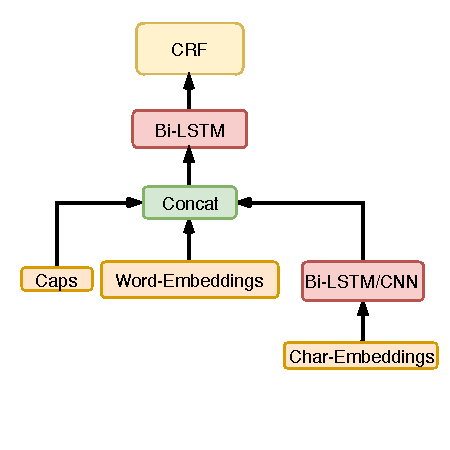
\includegraphics{blstm-crf}
    \caption{Model architecture}
    \label{fig:arch}
\end{figure}

\subsection{Input Features}
\begin{itemize}
    \item Word Embeddings: Glove 300d.
    \item Char Embeddings: random init.
    \item Capitalism: 4 kinds of types.
\end{itemize}
Except that, nothing else is used.

\subsection{Character-level Representation}
Here I use the same structure as described in \cite{e2ecrf2016}. But it doesn't work well on
this task. Another approach is using Bi-LSTM as feature extracter. Concat the forward and backward 
hidden vectors, we get the character representation.

\subsection{Bi-directional LSTM}
Here I use Bi-LSTM as word embeddings featue extracter.

\subsection{CRF}
After getting the output of word Bi-LSTM, we can use CRF to calculate the likelihood.

\section{Experiment}
In this section, I provide details about training the neural network. I implement the neural network using the TensorFlow~\cite{tf} framework~\footnote{https://github.com/HawkAaron/Clinical-Entity-Recognition}.
The computations for a single model are run on a GeForce GTX 1080 TI GPU.
I do grid search over several hyper parameters, such as optimizer, char embeddings, word embeddings, LSTM layers and CNN or LSTM.

\subsection{Grid Search Results}

Table~\ref{tab:grid} shows the results of difference models on development set. Here I only pick several best results.
There are over 20 models can get F1 score higher than 84.5 on dev set.
\begin{table}[tbh]
    \caption{Grid search results on development set}
    \label{tab:grid}
    \centering
    \begin{tabular}{c | c | c | c | c}
        \hline
        Model & Accuracy & Precision & Recall & F1 \\
        \hline
        rmsprop.cap-2.char-100-300.word-300-300.plstm-2 & 95.03 & - & - & 85.23 \\
        \hline
        adam.cap-5.char-50-100.word-300-300.plstm-2 & 95.00 & 84.90 & 85.28 & 85.01 \\
        \hline
        rmsprop.cap-2.char-50-300.word-300-100.plstm-3 & 94.85 & 85.47 & 84.51 & 84.99 \\
        \hline
        adam.char-20-300.plstm-1 & 94.85 & 85.47 & 84.51 & 84.99 \\
        \hline
    \end{tabular}
\end{table}

\subsection{Ensemble Training}
We select our best 20 models, with F1 score on dev set higher than 84.5, and then load them to a single graph and session.
For simplicity, we apply the method described in~\cite{ensemble}. The ensemble structure is shown in fig.~\ref{fig:ensemble}.

\begin{figure}[tbh]
    \centering
    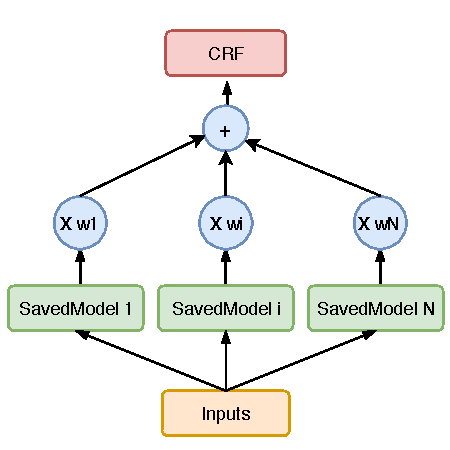
\includegraphics{ensemble_crf}
    \caption{Model architecture: inputs is the same with grid search section, we combine each saved model with differenct structure by multiplying a weight scalar. Each $w_i$ is a probability, and $\sum_i w_i = 1$. And the CRF transition matrix is averaged from saved models.}
    \label{fig:ensemble}
\end{figure}

We do ensemble training using difference combination of models and optimizers.
Since those saved model alreadly converged, so we only need one epoch to get the best score on ensemble training.
Note that the variables of saved models are not updated, we only update ensemble weights.

We first using 15 best models do ensemble training, and resuts are shown in table~\ref{tab:ensemble}.
We find that sgd can get the best score on dev set. Then we use all 20 best models do ensemble training, and the optimizer is sgd,
results are shown in table~\ref{tab:best}.
Finally, the F1 score on test set is shown in table~\ref{tab:final}.

% 15 models fusion
\begin{table}[tbh]
    \caption{Ensemble training results on development set using 15 best models}
    \label{tab:ensemble}
    \centering
    \begin{tabular}{c | c | c | c | c}
        \hline
        Optimizer & Accuracy & Precision & Recall & F1 \\
        \hline
        rmsprop & 95.29 & 86.92 & 85.18 & 86.04 \\
        \hline
        adam & 95.33 & 86.95 & 85.42 & 86.18 \\
        \hline
        adadelta & 95.47 & 86.87 & 86.27 & 86.57 \\
        \hline
        \bf{sgd} & \bf{95.58} & \bf{87.14} & \bf{86.31} & \bf{86.72} \\
        \hline
    \end{tabular}
\end{table}

% 20 models fusion
\begin{table}[tbh]
    \caption{Ensemble training results on \textbf{Dev} set using 20 best models}
    \label{tab:best}
    \centering
    \begin{tabular}{c | c | c | c}
        \hline
        Accuracy & Precision & Recall & F1 \\
        \hline
        \bf{95.65} & \bf{87.65} & \bf{86.07} & \bf{86.85} \\
        \hline
    \end{tabular}
\end{table}

% test result
\begin{table}[tbh]
    \caption{Ensemble training results on \textbf{Test} set using 20 best models}
    \label{tab:final}
    \centering
    \begin{tabular}{c | c | c | c}
        \hline
        Accuracy & Precision & Recall & F1 \\
        \hline
        \bf{94.72} & \bf{83.33} & \bf{85.55} & \bf{84.43} \\
        \hline
    \end{tabular}
\end{table}

\section{Analysis}
\subsection{Model Structure}
There are many differenct kinds of structure that we can use to do this task. 
For example, we can use the framework of encoder-decoder with attention to do sequence labelling~\cite{s2sner}.

\subsection{Ensemble Method}
Even using the naive ensemble approach described above, we can get significant improvement.
There is another method called knowledge distillation~\cite{ts}, can also achieve big improvement over normal trained models.

\begin{thebibliography}{3}
\bibitem{e2ecrf2016}
Ma, Xuezhe and Eduard H. Hovy. 
\textit{End-to-end Sequence Labeling via Bi-directional LSTM-CNNs-CRF}. 
CoRR abs/1603.01354 (2016): n. pag.

\bibitem{tf}
Martín Abadi, Ashish Agarwal, Paul Barham, Eugene Brevdo,
Zhifeng Chen, Craig Citro, Greg S. Corrado, Andy Davis,
Jeffrey Dean, Matthieu Devin, Sanjay Ghemawat, Ian Goodfellow,
Andrew Harp, Geoffrey Irving, Michael Isard, Rafal Jozefowicz, Yangqing Jia,
Lukasz Kaiser, Manjunath Kudlur, Josh Levenberg, Dan Mané, Mike Schuster,
Rajat Monga, Sherry Moore, Derek Murray, Chris Olah, Jonathon Shlens,
Benoit Steiner, Ilya Sutskever, Kunal Talwar, Paul Tucker,
Vincent Vanhoucke, Vijay Vasudevan, Fernanda Viégas,
Oriol Vinyals, Pete Warden, Martin Wattenberg, Martin Wicke,
Yuan Yu, and Xiaoqiang Zheng.
\textit{TensorFlow: Large-scale machine learning on heterogeneous systems},
2015. Software available from tensorflow.org.

\bibitem{ensemble}
Austin Waters and Yevgen Chebotar. 
\textit{Distilling Knowledge from Ensembles of Neural Networks for Speech Recognition},
InterSpeech 2016.

\bibitem{s2sner}
Zhu, Su and Kai Yu. “Encoder-decoder with focus-mechanism for sequence labelling based spoken language understanding.” 2017 IEEE International Conference on Acoustics, Speech and Signal Processing (ICASSP) (2017): 5675-5679.

\bibitem{ts}
Geoffrey Hinton and Oriol Vinyals and Jeffrey Dean.
\textit{Distilling the Knowledge in a Neural Network},
NIPS 2015.

\end{thebibliography}
\end{document}
